\documentclass{article}


% if you need to pass options to natbib, use, e.g.:
%     \PassOptionsToPackage{numbers, compress}{natbib}
% before loading neurips_2023


% ready for submission
\usepackage[preprint]{neurips_2023}


% to compile a preprint version, e.g., for submission to arXiv, add add the
% [preprint] option:
%     \usepackage[preprint]{neurips_2023}


% to compile a camera-ready version, add the [final] option, e.g.:
%     \usepackage[final]{neurips_2023}


% to avoid loading the natbib package, add option nonatbib:
%    \usepackage[nonatbib]{neurips_2023}


\usepackage[utf8]{inputenc} % allow utf-8 input
\usepackage[T1]{fontenc}    % use 8-bit T1 fonts
\usepackage{hyperref}       % hyperlinks
\usepackage{url}            % simple URL typesetting
\usepackage{booktabs}       % professional-quality tables
\usepackage{amsfonts}       % blackboard math symbols
\usepackage{nicefrac}       % compact symbols for 1/2, etc.
\usepackage{microtype}      % microtypography
\usepackage{xcolor}         % colors
\usepackage{graphicx}

\bibliographystyle{plain} % We choose the "plain" reference style


\title{Navigating Old School Runescape: Neurosymbolic Reinforcement Learning in a Rich and Dynamic MMORPG Environment}


% The \author macro works with any number of authors. There are two commands
% used to separate the names and addresses of multiple authors: \And and \AND.
%
% Using \And between authors leaves it to LaTeX to determine where to break the
% lines. Using \AND forces a line break at that point. So, if LaTeX puts 3 of 4
% authors names on the first line, and the last on the second line, try using
% \AND instead of \And before the third author name.


\author{%
  Chandler Stewart \\
  \texttt{cs111@illinois.edu} \\
  % examples of more authors
  % \And
  % Coauthor \\
  % Affiliation \\
  % Address \\
  % \texttt{email} \\
  % \AND
  % Coauthor \\
  % Affiliation \\
  % Address \\
  % \texttt{email} \\
  % \And
  % Coauthor \\
  % Affiliation \\
  % Address \\
  % \texttt{email} \\
  % \And
  % Coauthor \\
  % Affiliation \\
  % Address \\
  % \texttt{email} \\
}


\begin{document}


\maketitle


\begin{abstract}
  Traditional deep learning methods have achieved great success, and often surpass innate human ability in tasks such as image recognition/classification, natural language processing, and game playing. However, they rely on learning a mapping from given input to learned output. This representation makes them adept at interpolation, but fundamentally incapable of extrapolation without additional augmentation. Neurosymbolic techniques solve this problem by learning predicates capable of generalization beyond the training distribution. These techniques are ideal candidates for learning a domain that may have high variance, or when data is sparse. This paper details a novel environment for neurosymbolic reinforcement learning consisting of a large but discrete state and action space and the application of the Neural Logic Machines (NLM) framework to the environment. The specific experiment detailed is a simple grid world consisting of an agent and goal location. The agent is tasked with navigating to the goal location in the fewest number of steps while avoiding obstructions in the environment. The NLM model is able to learn a path to the goal, but training time is prohibitively long. The codebase for the project is available here:  https://github.com/chandlerstewart/nlm-2009scape
\end{abstract}


\section{Introduction}


Neurosymbolic learning is an emerging field that aims to combine the strengths of neural networks and symbolic reasoning. Neural networks are powerful function approximators that can learn from large amounts of data, but they often lack interpretability and generalization. Symbolic reasoning is a logic-based approach that can handle complex and abstract concepts, but it often requires human expertise and domain knowledge. By integrating neural and symbolic components, neurosymbolic learning can potentially achieve abstract reasoning and generalization from data.

One of the applications of neurosymbolic learning is reinforcement learning (RL), which is a framework for learning optimal policies from trial-and-error interactions with an environment. RL agents can benefit from neurosymbolic learning in several ways, such as incorporating prior knowledge, enhancing exploration, and improving transferability. However, designing and evaluating neurosymbolic RL agents is challenging, especially for domains that have high variance or sparse data.

In this paper, a novel environment for neurosymbolic RL is proposed that consists of a large but discrete state and action space. The environment is based on Old School Runescape (OSRS), a popular massively multiplayer online role-playing game (MMORPG) that features a rich and dynamic world with various tasks and quests. The focus is a simple grid world scenario within OSRS, where an agent has to navigate to a goal location while avoiding obstructions. NLMs are applied to the environment, and the results are discussed.


\section{Background}
\subsection{Reinforcement learning}
RL techniques aim to learn optimal policies from trial and error given a reward signal. \cite{sutton2018reinforcement}. RL agents can perform various tasks, such as playing games, controlling robots, and optimizing systems by maximizing a cumulative reward signal. However, they often face challenges such as high-dimensional state and action spaces, sparse and delayed rewards, and complex and dynamic environments. To overcome these challenges, RL agents require a generalizable and interpretable knowledge representation that can facilitate efficient learning and effective reasoning.

Markov decision processes (MDP) is a mathematical framework for modeling decision-making problems where the outcomes are partly random and partly controllable \cite{puterman2014markov}. An MDP consists of four components: a set of states S, a set of actions A, a transition function P that specifies the probability of moving from one state to another given an action, and a reward function R that specifies the immediate reward received after each transition. An MDP satisfies the Markov property, which means that the future state depends only on the current state and action.

\begin{figure}[h]
  
  \centering
  \fbox{
  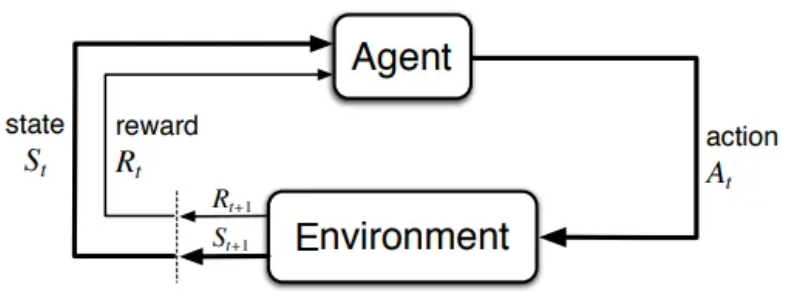
\includegraphics[scale=0.5]{imgs/mdp.png}
}
  
  \caption{Typical reinforcement learning cycle}
\end{figure}

A policy $\pi$ is a function that maps each state to an action or a distribution over actions. The goal of RL is to find an optimal policy $\pi^*$ that maximizes the expected return $G_t$, which is the total discounted reward from time step $t$ onwards. The value function $V^\pi(s)$ is the expected return starting from state $s$ and following policy $\pi$. The action-value function $Q^\pi(s,a)$ is the expected return starting from state $s$, taking action $a$, and following policy $\pi$ thereafter. The optimal value functions $V^*(s)$ and $Q^*(s,a)$ are the maximum values achievable by any policy.

There are different methods for finding optimal policies and value functions in RL, such as dynamic programming, Monte Carlo methods, and temporal difference learning. One of the most popular methods is the policy gradient method, which directly optimizes the policy by following the gradient of the expected return with respect to the policy parameters \cite{sutton1999policy}. Policy gradient methods can handle continuous action spaces and stochastic policies, and they are often combined with function approximation techniques such as neural networks.
One of the simplest policy gradient methods is REINFORCE \cite{williams1992simple}, which is a Monte Carlo variant of a policy gradient algorithm. REINFORCE uses a neural network to represent the policy $\pi_\theta(a|s)$, where $\theta$ are the network parameters. 

REINFORCE collects samples of an episode using its current policy, and uses them to update $\theta$ by gradient ascent:

\begin{equation}
\theta \leftarrow \theta + \alpha G_t \nabla_\theta \ln \pi_\theta(a_t|s_t)
\end{equation}

where $\alpha$ is the learning rate, $G_t$ is the total discounted reward from time step $t$ onwards, and $\frac{\partial}{\partial \theta} \ln \pi_{\theta}(a_t|s_t)$ is the gradient of the log-probability of taking action $a_t$ in state $s_t$ under the policy $\pi_{\theta}$. REINFORCE can learn effective policies from raw data, but it has high variance and slow convergence. There are various extensions and improvements of REINFORCE, such as adding a baseline or a critic to reduce variance, using multiple parallel agents to collect more data, or using an actor-critic architecture to combine policy gradient and value function methods.

\subsection{Neurosymbolic learning}

Neurosymbolic learning is an emerging field that combines the strengths of neural networks and symbolic reasoning \cite{garcez2019neural}. Neural networks have shown great performance when interpolating within their trained distribution but they often lack interpretability and generalization. Symbolic reasoning is a logic-based approach that can handle complex and abstract concepts, but it often requires human expertise and domain knowledge. By integrating neural and symbolic components, neurosymbolic learning can potentially achieve both data-driven and knowledge-driven learning, as well as provide explanations for the learned models.

\subsubsection{Neural Logic Machines}

Neural Logic Machines (NLMs) are a neurosymbolic architecture that has gained attention in recent years \cite{dong2019neural}. NLMs combine neural networks and logic-based reasoning to enable learning, reasoning, and planning. They consist of two main components: a neural module and a logic module. The neural module learns latent representations of objects and relations from the data, capturing important features and patterns. The logic module learns logic rules over these latent representations, allowing for symbolic reasoning and inference.When trained for RL, the standard algorithm used for policy optimization is REINFORCE \cite{williams1992simple}.

The neural module of NLMs leverages neural networks to process and learn from data. It can be designed using various neural architectures, such as convolutional neural networks (CNNs) or recurrent neural networks (RNNs), depending on the nature of the input data and the specific task at hand. The neural module's role is to extract useful features and encode them into a representation that captures the underlying relationships between objects and their attributes. It learns logic rules that operate on the latent representations, enabling deductive reasoning and inference. The logic rules can be learned using various techniques, such as inductive logic programming or differentiable logic, which allow for the integration of logical reasoning with gradient-based learning.

\begin{figure}[h]
  
  \centering
  \fbox{
  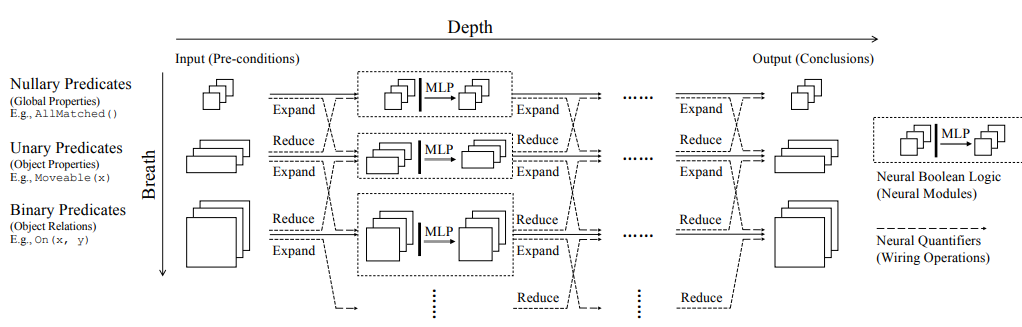
\includegraphics[scale=0.5]{imgs/nlm.png}
}
  
  \caption{Neural Logic Machine architecture \cite{dong2019neural}}

\end{figure}


NLMs can perform both inductive learning, where they learn patterns and generalizations from data, and deductive reasoning, where they use logic rules to draw conclusions based on the learned knowledge. Additionally, NLMs can handle uncertainty and compositionality, allowing them to reason with incomplete or noisy data and to combine learned concepts to solve more complex problems.

NLMs have been tested on several different domains. They have been successfully applied to family tree reasoning, where they can infer relationships and answer questions about kinship based on the available information. They have also been used for block stacking tasks, where they can learn to stack blocks based on their attributes and spatial relations.
\section{Motivation}

Traditional RL algorithms are very effective at converging to an optimal policy, but they often do not generalize well to unseen environments. Few frameworks exist for RL training, and their capabilities are relatively unexplored. NLMs are a promising approach for application to more interesting and complex problems. The existence of a suitable environment for training NLMs and other neurosymbolic architectures would be a significant step forward in the field of neurosymbolic learning.

\section{Related Work}

\subsection{Logic Networks}

Logical Neural Networks (LNNs) introduces a weighted real-valued logic that assigns meanings to every neuron as a component of a logical formula, resulting in a highly interpretable and disentangled representation. The network is also end-to-end differentiable. LNNs are a promising approach to neurosymbolic learning, but application to RL is difficult due to requiring a definition of the logical rules beforehand. \cite{sen2021neurosymbolic} use LNNs to induce a logical representation of a policy, but they have not released their code, making it difficult to reproduce their results. Logic Tensor Networks (LTNs) \cite{serafini2016logic} are similar to LNNs, but use Real Logic as opposed to first-order.

\subsection{Relational Reinforcement Learning}

Relational reinforcement learning aims to enhance RL agents by incorporating relational representations and reasoning. A framework with the same name: Relational reinforcement learning (RRL) combines reinforcement learning with relational learning and reasoning \cite{dzeroski2001relational}. RRL agents learn from relational data, such as graphs or knowledge bases, and use relational representations to generalize to unseen environments. RRL has been applied to various domains, such as robotics, natural language processing, and computer vision. For example, RRL has been used to learn relational policies for robotic manipulation tasks, enabling agents to generalize to new objects and environments. RRL has also been applied to natural language processing tasks, such as question answering and machine translation, where it can learn to reason about the relationships between words and sentences.


\subsection{Multi-modal Neurosymbolic Learning}
The integration of multi-modal data, such as images and text, has been an active area of research in neurosymbolic learning. Several works have explored combining neural networks with symbolic reasoning for tasks that require reasoning over both visual and textual information. For instance, Visual Question Answering (VQA) tasks involve answering questions about images, which require both visual perception and language understanding. Neurosymbolic approaches have been proposed for VQA tasks, leveraging neural networks for image processing and symbolic reasoning to handle question semantics and relationships between visual elements \cite{hu2017learning}.

\section{Old School Runescape Environment}

\begin{figure}[h]
  
  \centering
  \fbox{
  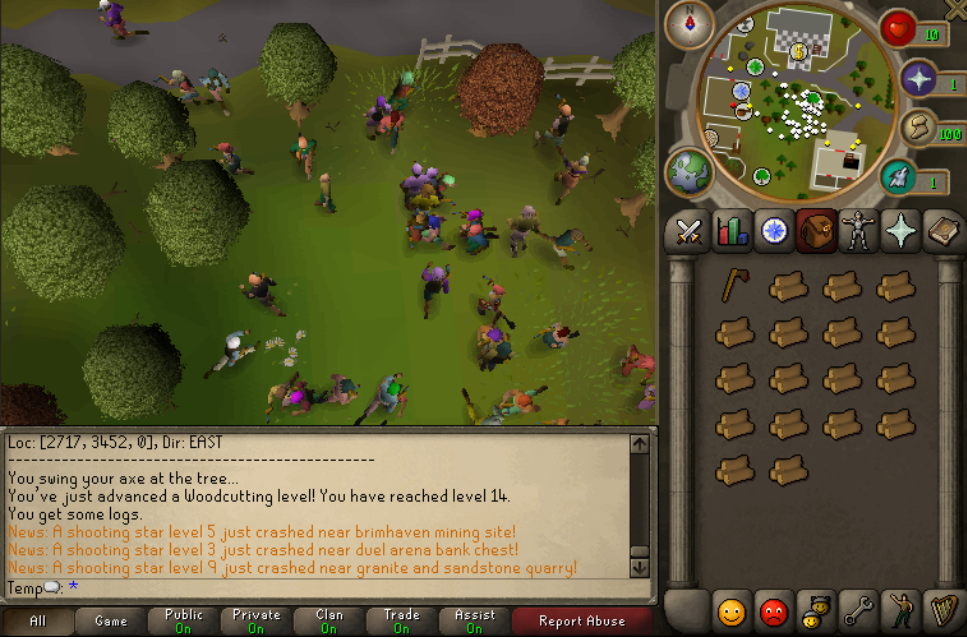
\includegraphics[scale=0.5]{imgs/game2.png}
}
  
  \caption{Old School Runescape Training Environment. The bots are learning to navigate the environment.}
\end{figure}


\subsection{Overview}



Old School Runescape (OSRS) is a popular massively multiplayer online role-playing game (MMORPG) that features a rich and dynamic world with various tasks and quests. OSRS is based on Runescape as it was in 2007, and it has been maintained by the community since 2013. OSRS provides a novel environment for neurosymbolic RL, as it has a large but discrete state and action space, a diverse set of scenarios and objectives, and a realistic and immersive setting. Numerous tasks and quests in OSRS require reasoning and planning, such as navigating complex environments or solving puzzles.

In OSRS, players can create a character and explore the world of Gielinor. Players can interact with the environment by moving around, talking to non-player characters, and performing various actions such as mining, fishing, and cooking. Players can also fight monsters and other players in player-versus-environment and player-versus-player (PvP) combat. Players can gain experience points (XP) by performing actions, and level up their skills by gaining enough XP. Players can also complete quests to gain XP and unlock new areas, items, and abilities. There are various skills and quests in OSRS, such as mining, fishing, cooking, woodcutting, firemaking, smithing, crafting, magic, and combat.

From the reinforcement learning perspective, OSRS is a partially observable Markov decision process with a large but discrete state and action space. The reward function is an interesting challenge, as there are many different ways to play OSRS, different goals to pursue, and different ways to achieve those goals. A sparse reward signal could be used to encourage exploration, or a dense reward signal could be used to guide the agent towards a specific goal. It also could lead to emergent behavior, such as the agent learning to trade with other players or join clans to gain XP and items.

Due to the large state and action space, the complex environment, and the diverse set of tasks and quests, OSRS could be a challenging environment for neurosymbolic RL. It could be used to study various aspects of neurosymbolic learning, such as learning predicates from data, learning logic rules from data, and combining neural and symbolic components. Other potential applications include the study of multi-modal reinforcement learning,multi-agent learning, and domain generalization.

\subsection{State and Action Space}
The state space of OSRS is composed of three main components: the game world, the player's inventory, and the player's skills. The game world is a large and diverse map that contains over 50 regions, each with its own terrain, climate, and features. The game world has more than 15,000 tiles, which are the basic units of movement and interaction. Each tile can have one or more objects on it, such as trees, rocks, chests, or doors. The game world also has many non-player characters (NPCs) and other players that can interact with the player or each other. The player's inventory is a limited storage space that can hold up to 28 items, such as weapons, armor, food, or potions. The player's skills are numerical attributes that represent the player's proficiency in various activities, such as combat, magic, crafting, or fishing. There are 23 skills in OSRS, and each skill can range from level 1 to level 99.

The action space of OSRS is defined by the player's movements and interactions. The player can move in any direction and across any tile that is not blocked by an object or a boundary. The player can also interact with any object, NPC, or other player that is within their reach. The type and effect of the interaction depend on the object or character involved, as well as the player's inventory and skills. For example, the player can chop down a tree to obtain logs, talk to a shopkeeper to buy or sell items, cast a spell to damage an enemy or heal an ally, or trade items with another player. The action space of OSRS is large and diverse, and it allows for many different strategies and outcomes.


\section{Methodology}

\subsection{State Representation and Actions}

The state space consists of a 5x5 grid centered on the agent. 5 predicates are used to represent the state space: TileBlocked(x,y), GoalNorth(x,y), GoalSouth(x,y), GoalEast(x,y), and GoalWest(x,y). The TileBlocked predicate is true if the tile is blocked by an object or a boundary. The GoalNorth, GoalSouth, GoalEast, and GoalWest predicates are true if the goal is in the corresponding direction with repsect to each tile. Because the state space is partially observable, the agent must learn to reason about the environment and plan its actions accordingly. The nearest 25 tiles are observed, and the agent must learn to infer the state of the rest of the environment.

One action is available for the agent, Move(x,y). Given the x,y coordinates of one tile in the 5x5 grid, the agent moves to that tile. The agent can only move to tiles that are not blocked by an object or a boundary. 

\begin{figure}[h]
  
  \centering
  \fbox{
  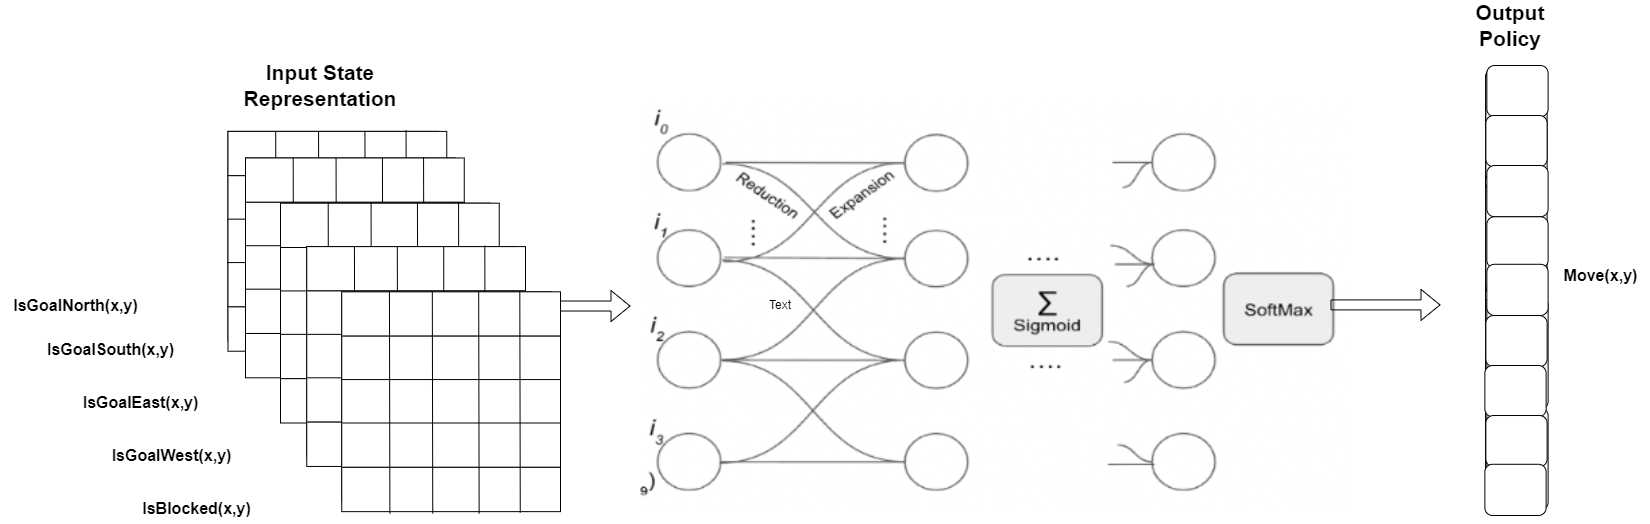
\includegraphics[scale=0.25]{imgs/state.png}
}
  
  \caption{Input to the Neural Logic Network and the corresponding output. The agent is located at the center of the 5x5 grid. }
\end{figure}

\subsection{Reward Function}

Due to the complexity and partial observability of the environment, reward shaping is used to make the problem of learning a path tractable. The agent is provided a reward every step based on the manhattan distance between the agent and the goal compared to the manhattan distance between the start location and the goal (Equation 2). The agent is also provided an additional large reward as it reaches the goal.

\begin{equation}
    r = |x_{goal} - x_{start}| + |y_{goal} - y_{start}| - |x_{goal} - x_{agent}| + |y_{goal} - y_{agent}|
\end{equation}


\subsection{Experiment Setup}

A static start and goal location is chosen. Approximately 20 tiles away based on the manhattan distance. The agent is trained using a Neural Logic Network with a depth of 9 and breadth of 2. The depth and breadth parameters define the number of layers in the model and the arity of the predicates, respectively. The network is trained using the Adam optimizer with a learning rate of 0.005. The model was trained for approximately four hours with the following hardware:

\begin{itemize}
    \item CPU: AMD EPYC™ 7543P CPU with 4 cores and 8 threads
    \item GPU: NVIDIA® RTX™ A4500
    \item RAM: 28 GB
\end{itemize}

\section{Results}

\begin{figure}[h]
\centering
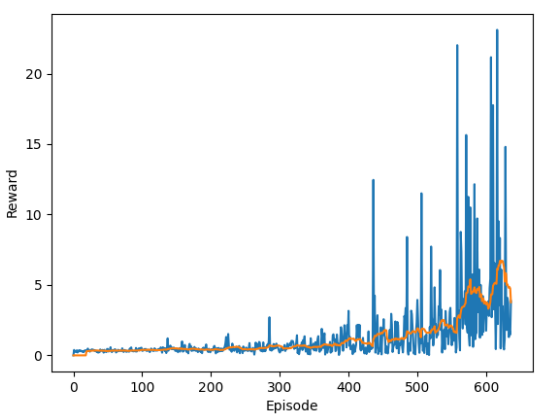
\includegraphics[width=0.75\textwidth]{imgs/plot1.png}
\caption{Reward over time. The blue line denotes the value for each episode. The orange line denotes the average value over the last 20 episodes.}
\end{figure}

Figure 2 shows the reward over time for the agent. The agent is able to learn a path to the goal, but it is not able to learn the optimal path. NLMs is an expensive algorithm, as a result, the model's learning seems to be still converging. No baselines were used for comparison, as the goal of this project was to explore the capabilities of NLMs in a novel environment using a relational state representation. Generalization to new start and goal locations was not tested, but the partial observability of the environment and success of the agent in learning a path to the goal suggests that the agent could generalize to new start and goal locations.

\section{Future Work}
The primary challenge of NLMs is the scalability of the algorithm. The authors of the original paper noted in an online discussion post that they trained on a smaller environment representation using 12 CPUs and a 1080 TI GPU. Therefore, this is an obvious place for improvement. Another concern is the nature of the learned policy. While it is dervied from a set of logically induced rules, the policy itself does not have a symbolic representation. Therefore, a possible direction for future research is to explore methods for making the policy more explicit and interpretable, such as using attention mechanisms or rule extraction techniques. Another potential avenue for improvement is to investigate the use of sparse reward signals, which could foster exploration and emergent behavior in NLMs. Given the nature of logical rules, it is conceivable that the agent could learn a hierarchy of rules, where it builds on simpler rules to infer more complex ones.

\section{Conclusion}

NLMs are a lesson in the capabilities of neuralsymbolic architectures, but are infeasible for larger environments. However, they are a promising direction for future research, and they could be used to study various aspects of neurosymbolic learning, such as learning predicates from data, learning logic rules from data, and combining neural and symbolic components. Other potential applications include the study of multi-modal reinforcement learning, exploration, sparse rewards, multi-agent learning, and domain generalization.


\bibliography{references.bib}

\appendix

\section{Appendix}
\subsection{Deviation From Original Proposal}

The original proposal was to induce a symbolic representation from a learned policy from an established traditional reinforcement learning technique to obtain a symbolic representation of a policy. However, the essence of a policy is a mapping from states to actions, which can be simply represented by a set of logical rules. This representation would lose information, as the decision making process learned from numerous sets of positive and negative examples would be reduced to a set of rules constrained to the training data. Therefore, the focus of the project was shifted to the more interesting problem of utilizing an established neurosymbolic framework to solve a challenging task, explore the limitations of the framework, and build an environment for diverse neurosymbolic reinforcement learning research.

\subsection{Environment Implementation Details}

The environment is an open-source remake of the popular game Old School Runescape. It is coded in Java and was modified to support socket data transfer. The environment can be run locally or on a remote server, and it can be accessed via a Python client. It is designed to be modular and extensible, so it can be easily modified to support new features and scenarios. Currently, it is a minimal implementation that supports basic movement and interaction, but it could be expanded to support more complex scenarios and tasks.

\end{document}